% !TEX root =  master.tex
\section{Implementierung des Saalplans}
\authorsection{\authorNL}

\subsection{Darstellung des Kinosaals}

Eine zentrale Aufgabe im Front-End war es, den Kinosaal mit den Sitzen anzuzeigen und dem Benutzer zu ermöglichen, Plätze auszuwählen.

Dies lässt sich mit einfachen Mitteln auch in \acs{HTML} umsetzen, z.B. mit \textit{div}-Elementen, bei denen man Größe und Farbe festlegt.
Mit JavaScript wird dann implementiert, was passiert wenn ein Sitzplatz angeklickt wird.

\begin{figure}[ht]
	\centering
	\subfloat{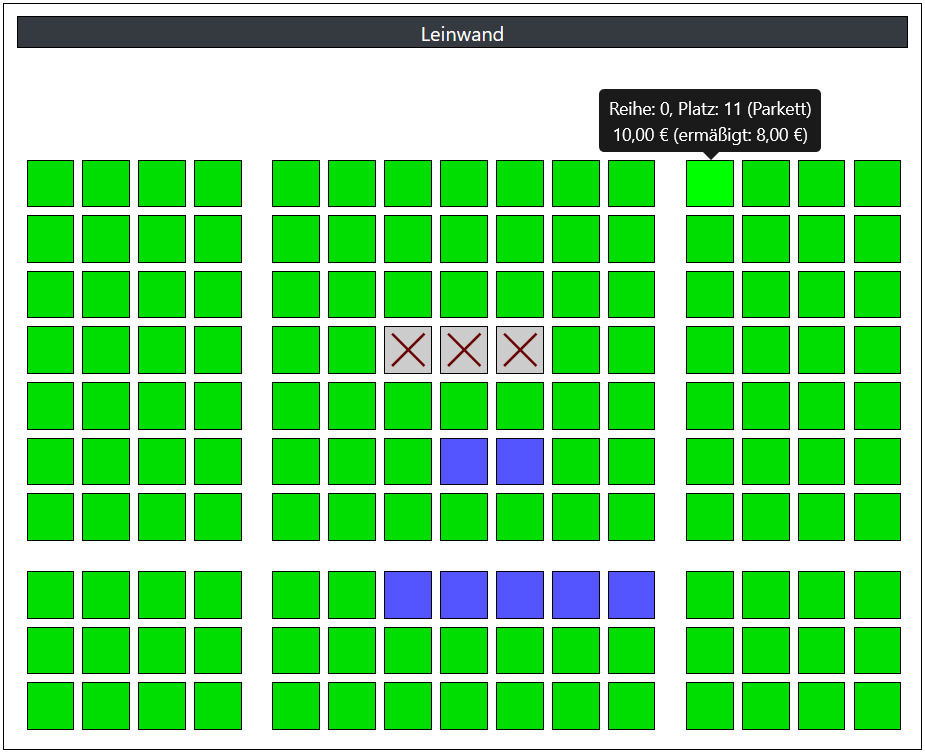
\includegraphics[height=0.295\textheight]{img/screenshots/saalplan01}}
	\hfill
	\subfloat{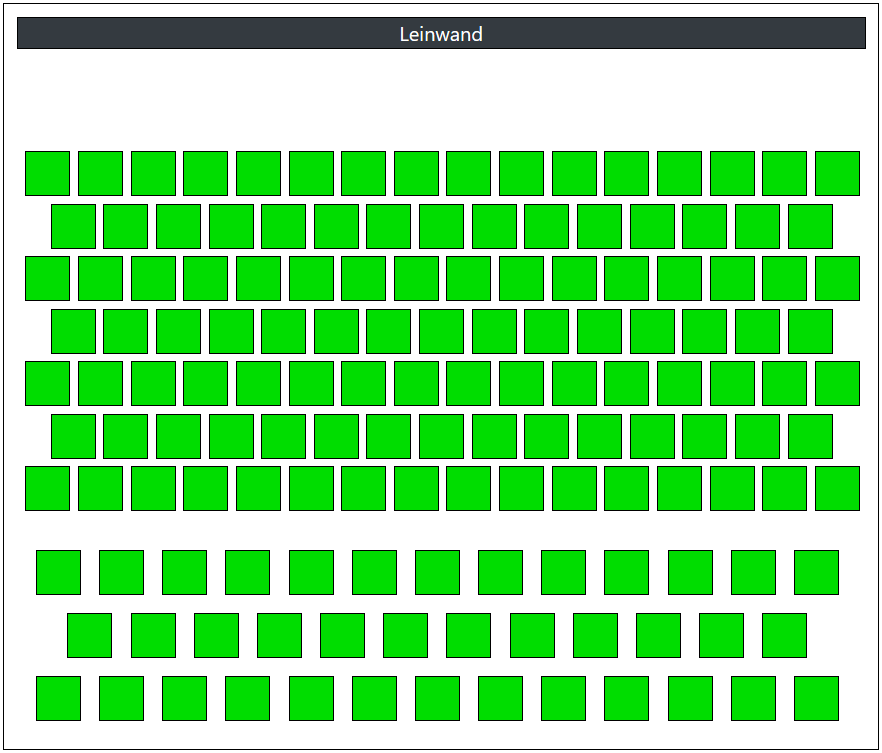
\includegraphics[height=0.295\textheight]{img/screenshots/saalplan03}}

	\caption{Saalpläne}
	\label{fig:saalplan}
\end{figure}

In Abbildung \vref{fig:saalplan} kann man sehen, wie der Kinosaal im Browser dargestellt wird.
Eine Box außen bildet die Umrandung und stellt den Saal dar.
Darin befindet sich eine zweite farblich hervorgehobene Box, die die Leinwand abbildet, damit die Benutzer wissen, wo im Kinosaal vorne und hinten ist, und sie somit ihre Entscheidung, wo sie sitzen möchten, treffen können.
Darunter finden sich dann die Sitzplätze.

Die Sitzplätze sind dabei farblich gekennzeichnet, um anzuzeigen, ob ein Sitzplatz frei oder belegt ist.
Belegte Sitze sind einerseits grau, andererseits auch noch mit einem Kreuz versehen, um Menschen, die in ihrer Farbwahrnehmung eingeschränkt sind, zu berücksichtigen.
Außerdem werden ausgewählte Sitze blau markiert und der Sitz, über dem aktuell die Maus ist, wird ebenso hervorgehoben.
Ein Tooltip mit einer kurzen Beschreibung und Details zu Kategorie und Preis, gibt dem Benutzer weitere Informationen.

Das Aussehen der Sitzplätze wird über Klassen und eine eigene \acs{CSS}-Datei definiert, sodass sich dies schnell anpassen lässt und zum Beispiel die Farbe der Sitzplätze mit einem Mal änderbar ist.

\begin{figure}[ht]
	\centering
	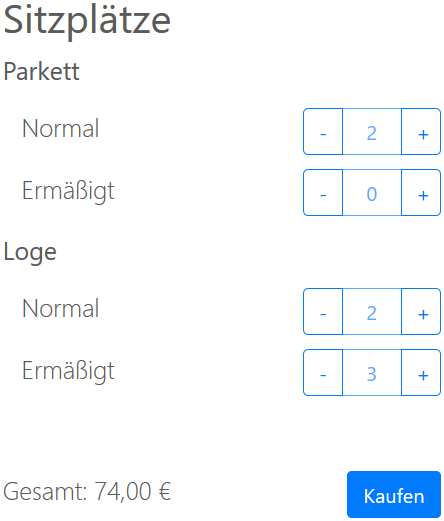
\includegraphics[width=0.4\textwidth]{img/screenshots/saalplan02}
	\captionsetup{format=hang}
	\caption{Preisstufen}
	\label{fig:saalplan02}
\end{figure}

Wählt man nun Sitzplätze aus, so muss man noch angeben, wie viele Tickets zum normalen Preis man kaufen möchte und wie viele zu einem ermäßigten Preis.
Daraus wird dann direkt der Preis berechnet und angezeigt (siehe Abbildung \ref{fig:saalplan02}).
Je nach Bildschirmgröße und -dimensionen werden diese Element neben dem Saalplan oder darunter angezeigt.
Mit dem \enquote{Kaufen}-Button gelangt man dann zur nächsten Seite, um weitere Daten anzugeben.

In der ersten Implementierung wurden der Saal und die Sitzplätze mit absoluten Größenangaben definiert.
So hatte das \textit{div}-Element, das einen Sitzplatz darstellt, als Höhe und Breite \textit{20px} gesetzt und eine Position relativ zur links oberen Ecke des Saals in Pixeln angegeben.
Die Koordinaten kommen dabei direkt aus dem Back-End bzw. der Datenbank.
Dies ermöglicht es, nicht nur einfach alle Plätze nebeneinander anzuzeigen, sondern auch Gänge einzufügen, Plätze versetzt anzuordnen, die Abstände zwischen den Sitzen individuell zu gestalten und somit den Saalplan an die Realität anzupassen.

Durch die Verwendung absoluter Größen in Pixeln, ist jedoch das Benutzererlebnis auf kleinen Bildschirmen schlechter.
Der Saal ist erst einmal breiter als der Bildschirm und der Benutzer muss herauszoomen und die Größe selbst anpassen.
Das Gleiche gilt für Benutzer eines Desktop-Computers, wenn sie die Fenstergröße anpassen.

Um dies zu verbessern, wird beim erstmaligen Laden sowie bei jeder Änderung der Fenstergröße, die Größe des Saals und der Sitzplätze neu berechnet.
Die Größenangaben aus der Datenbank werden dabei genutzt und entsprechend skaliert, sodass der Saalplan weder die volle Breite, noch die volle Höhe des Bildschirms überschreitet.
Um den Berechnungsaufwand zu reduzieren, sind die Koordinaten aller Sitzplätze prozentual angegeben.
Diese prozentualen Angaben beziehen sich dabei auf den \textit{div}-Container, der den Saal darstellt.
Dementsprechend muss lediglich die Größe des Saals und die Größe der Sitzplätze berechnet werden.

Ein Sitzplatz wird durch eine \acs{HTML}-Vorlage erstellt.
Die aus der Datenbank stammenden und in JavaScript verarbeiteten Werte werden zunächst in die Vorlage und im Anschluss ins \acs{DOM} eingefügt.

\begin{lstlisting}[style=lstHTML, caption={\acs{HTML}-Vorlage für die Darstellung eines Sitzplatzes}, label={lst:html_template_seat}]
<div id='`\textcolor{red}{\{seatID\}}`'
	class='seat `\textcolor{red}{\{classes\}}`'
	style='left: `\textcolor{red}{\{posx\}}`%; top: `\textcolor{red}{\{posy\}}`%;'
	title='`\textcolor{red}{\{tooltip\}}`'>
</div>
\end{lstlisting}

Die Gestaltung erfolgt dabei vollkommen über \acs{CSS}-Klassen, die in JavaScript hinzugefügt oder entfernt werden.

\begin{lstlisting}[style=lstCSS, caption={Optische Gestaltung der Sitzplätze}, label={lst:css_seat}]
.seat {
	border: 1px solid black;
}
.available {
	background-color: #0d0;
}
.occupied {
	background-color: #ccc;
}
.hovering {
	background-color: #0f0;
}
.selected {
	background-color: #55f;
}
\end{lstlisting}

\subsection{Reaktion auf Benutzerinteraktion}

Sobald der Benutzer einen Sitzplatz anklickt, wird diese Information an die zugehörige Funktion weitergereicht.

\begin{lstlisting}[language=JavaScript, caption={Erkennen des Anklickens eines Sitzplatzes}, label={lst:js_onclick}]
$(".seat").on("click", function () {
	var seatId = $(this).attr("id");
	if (seatId in selection) {
		removeSeatFromSelection(seatId, this);
	}
	else {
		addSeatToSelection(seatId, this);
	}
});
\end{lstlisting}

Wenn der Benutzer einen Sitzplatz auswählen möchte, muss noch einmal überprüft werden, ob dieser auch wirklich noch frei ist.
Zusätzlich soll der Sitzplatz für den Benutzer vorgemerkt werden, damit in der Zwischenzeit kein anderer den Sitzplatz reserviert.

Dafür wird eine \acs{AJAX}-Anfrage an das Back-End gesendet.
Dabei wird einerseits die Vorstellung und der ausgewählt Sitzplatz mitgegeben, andererseits aber auch eine Benutzeridentifizierung in Form einer zufälligen Zeichenkette, die im Browser des Benutzers als Cookie gespeichert wird.

\begin{lstlisting}[language=JavaScript, caption={Senden einer Anfrage, den Sitzplatz zu blocken}, label={lst:js_ajax_send_block}]
function addSeatToSelection (seatId, seatObj) {
	// prepare data for ajax
	var block = {show: {id: urlparameters.get("id")},
		seat: {id: seatId},
		sessiontoken: cookie};

	// send ajax
	var data = "block=" + JSON.stringify(block);
	$.ajax({
		type: "POST",
		url: "http://localhost:8080/cinema-system/reservation/block",
		data: data,
		contentType: "application/json; charset=utf-8",
		success: (data) => processBlockingResult(data, seatId, seatObj),
		error: function (xhr,status,error){
			console.log(xhr, status, error);
			processBlockingResult(null, seatId, seatObj);
		}
	});
}
\end{lstlisting}

Die Antwort des Servers wird an die entsprechende Funktion weitergegeben.
Dort wird nun überprüft, ob das Blocken des Sitzplatzes erfolgreich war oder nicht.

\begin{lstlisting}[language=JavaScript, caption={Verarbeiten der Server-Antwort beim Versuch, einen Platz zu blocken}, label={lst:js_ajax_process_block}]
function processBlockingResult (data, seatId, seatObj) {
	if(data != null) {
		var seatIdResponse = data.seat.id;
		seats[seatId].isBlocked = false;
		$(seatObj).addClass("selected available");
		$(seatObj).removeClass("occupied");
		selection[seatIdResponse] = true;
		numberOfTickets[getCategoryOfSeat(seatIdResponse)] += 1;
		updatePriceBox();
	} else {
		seats[seatId].isBlocked = true;
		$(seatObj).removeClass("available hovering");
		$(seatObj).addClass("occupied");
	}
}
\end{lstlisting}

Zum einen werden alle nötigen Variablen aktualisiert, zum anderen wird die Benutzeroberfläche entsprechend angepasst.
Dies umfasst den angeklickten Sitz selbst und auch die in Abbildung \vref{fig:saalplan02} gezeigten Auswahlmöglichkeiten für die Ermäßigung und Preisstufen der Sitzplätze.
